\documentclass[a4paper]{article}
\usepackage[letterpaper,top=2cm,bottom=2cm,left=3cm,right=3cm,marginparwidth=1.75cm]{geometry}
\usepackage[colorlinks=true, allcolors=blue]{hyperref}

\usepackage{wrapfig}
\usepackage{amsthm}
\usepackage{hyperref}
\usepackage{graphicx}
\usepackage{amsfonts}

\title{CUDA HW2}
\author{Patryk Drozd}
\begin{document}
\date{}
\maketitle

\section{Task1}

    Task 1 is done in files task1.c and task1\_funcs.c

\section{Task2}

	\begin{figure}[h!]
		\centering
		% 2048 4096 8192
		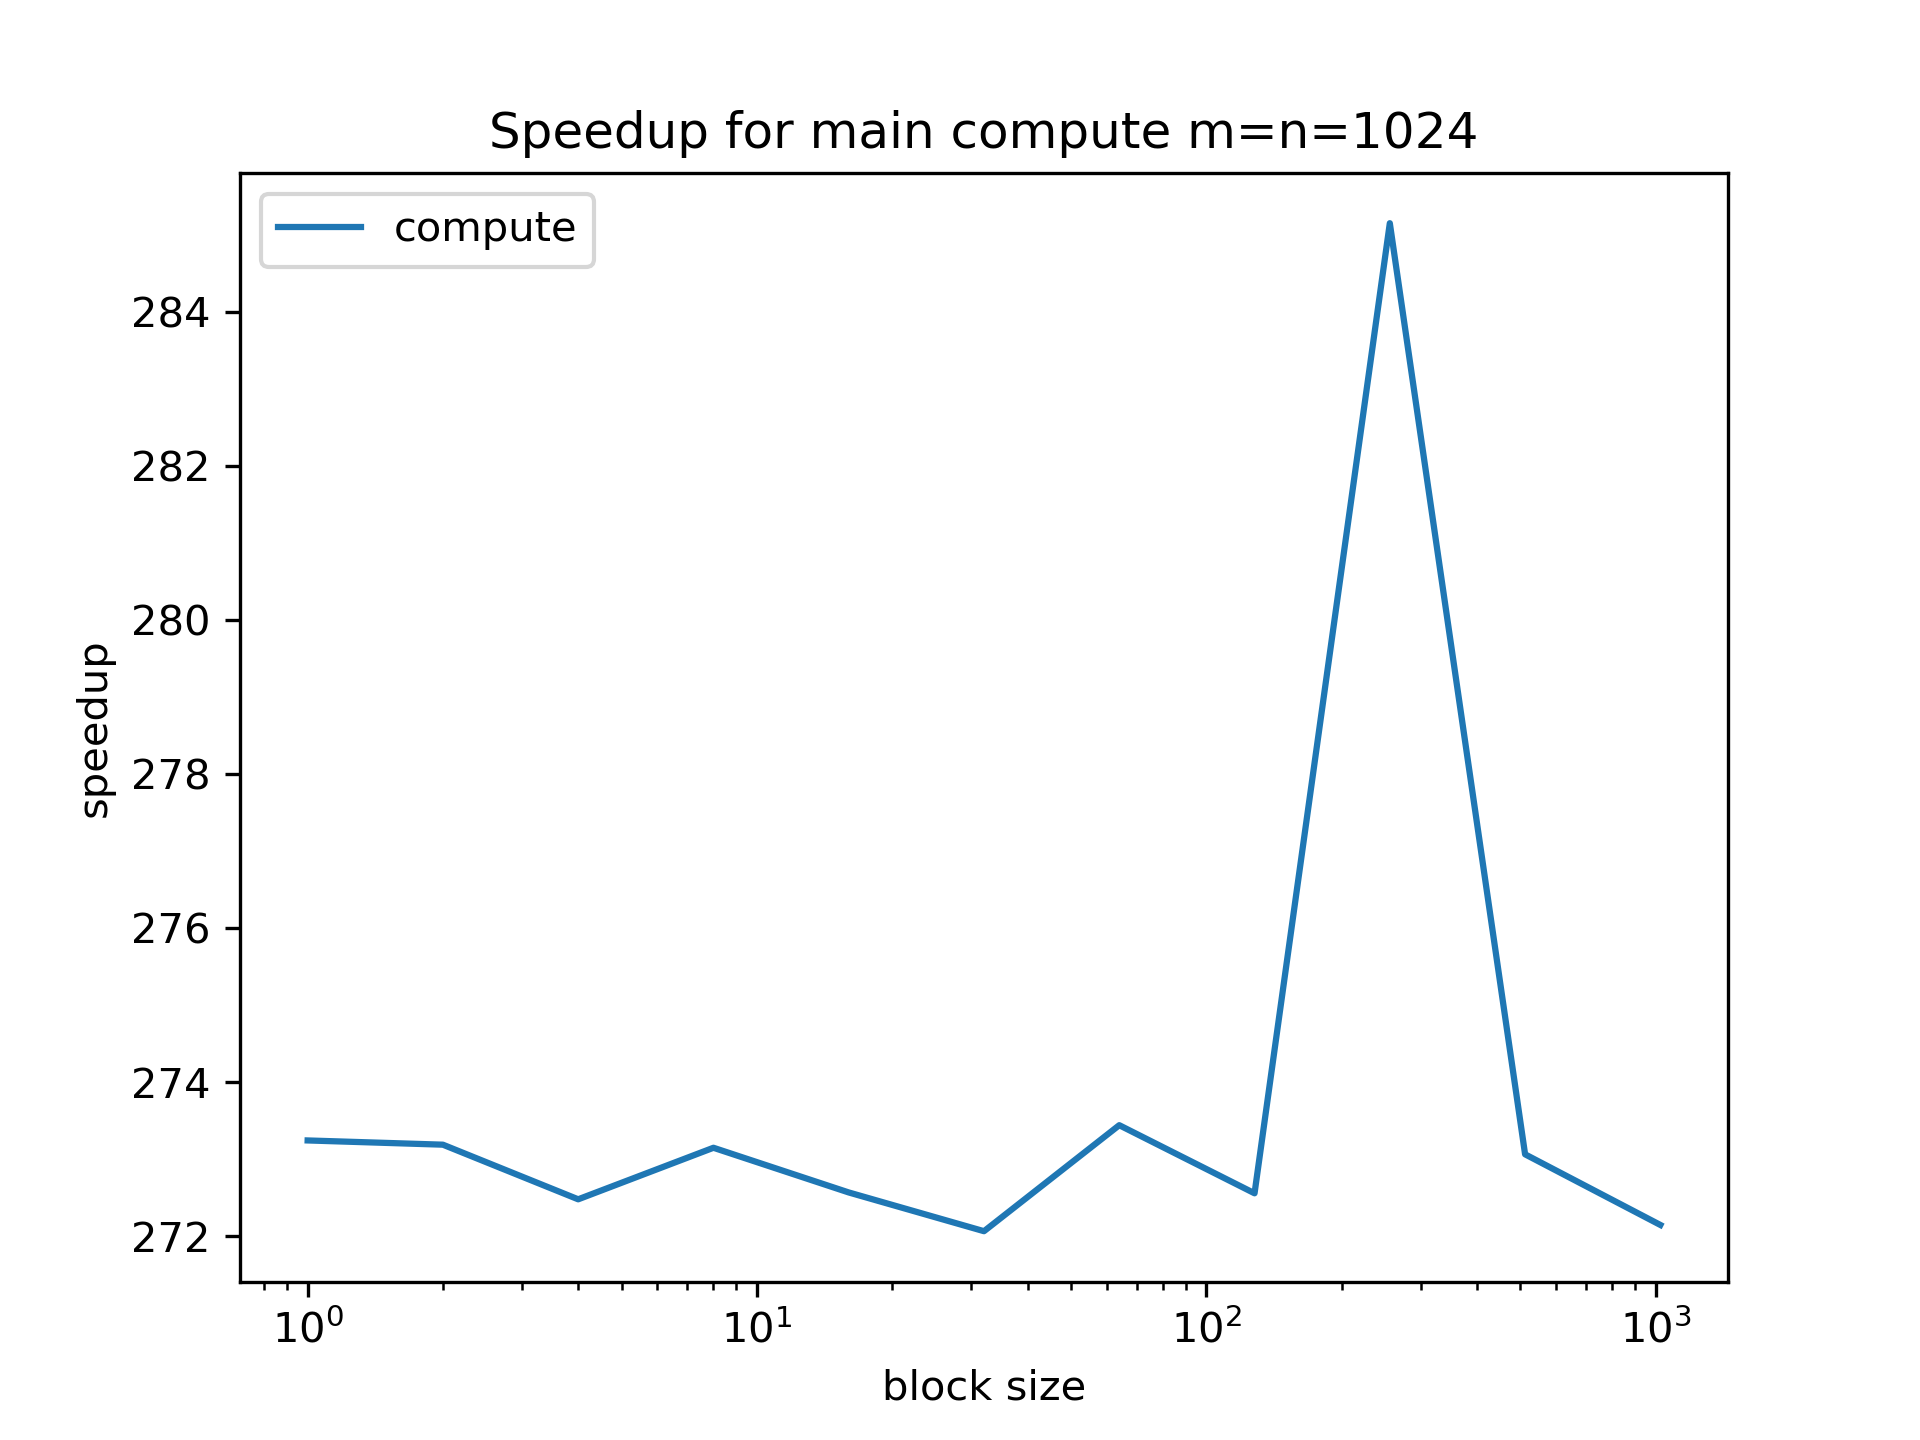
\includegraphics[width=.5\linewidth]{../float/writeup/compute_plot_m1024.png}
		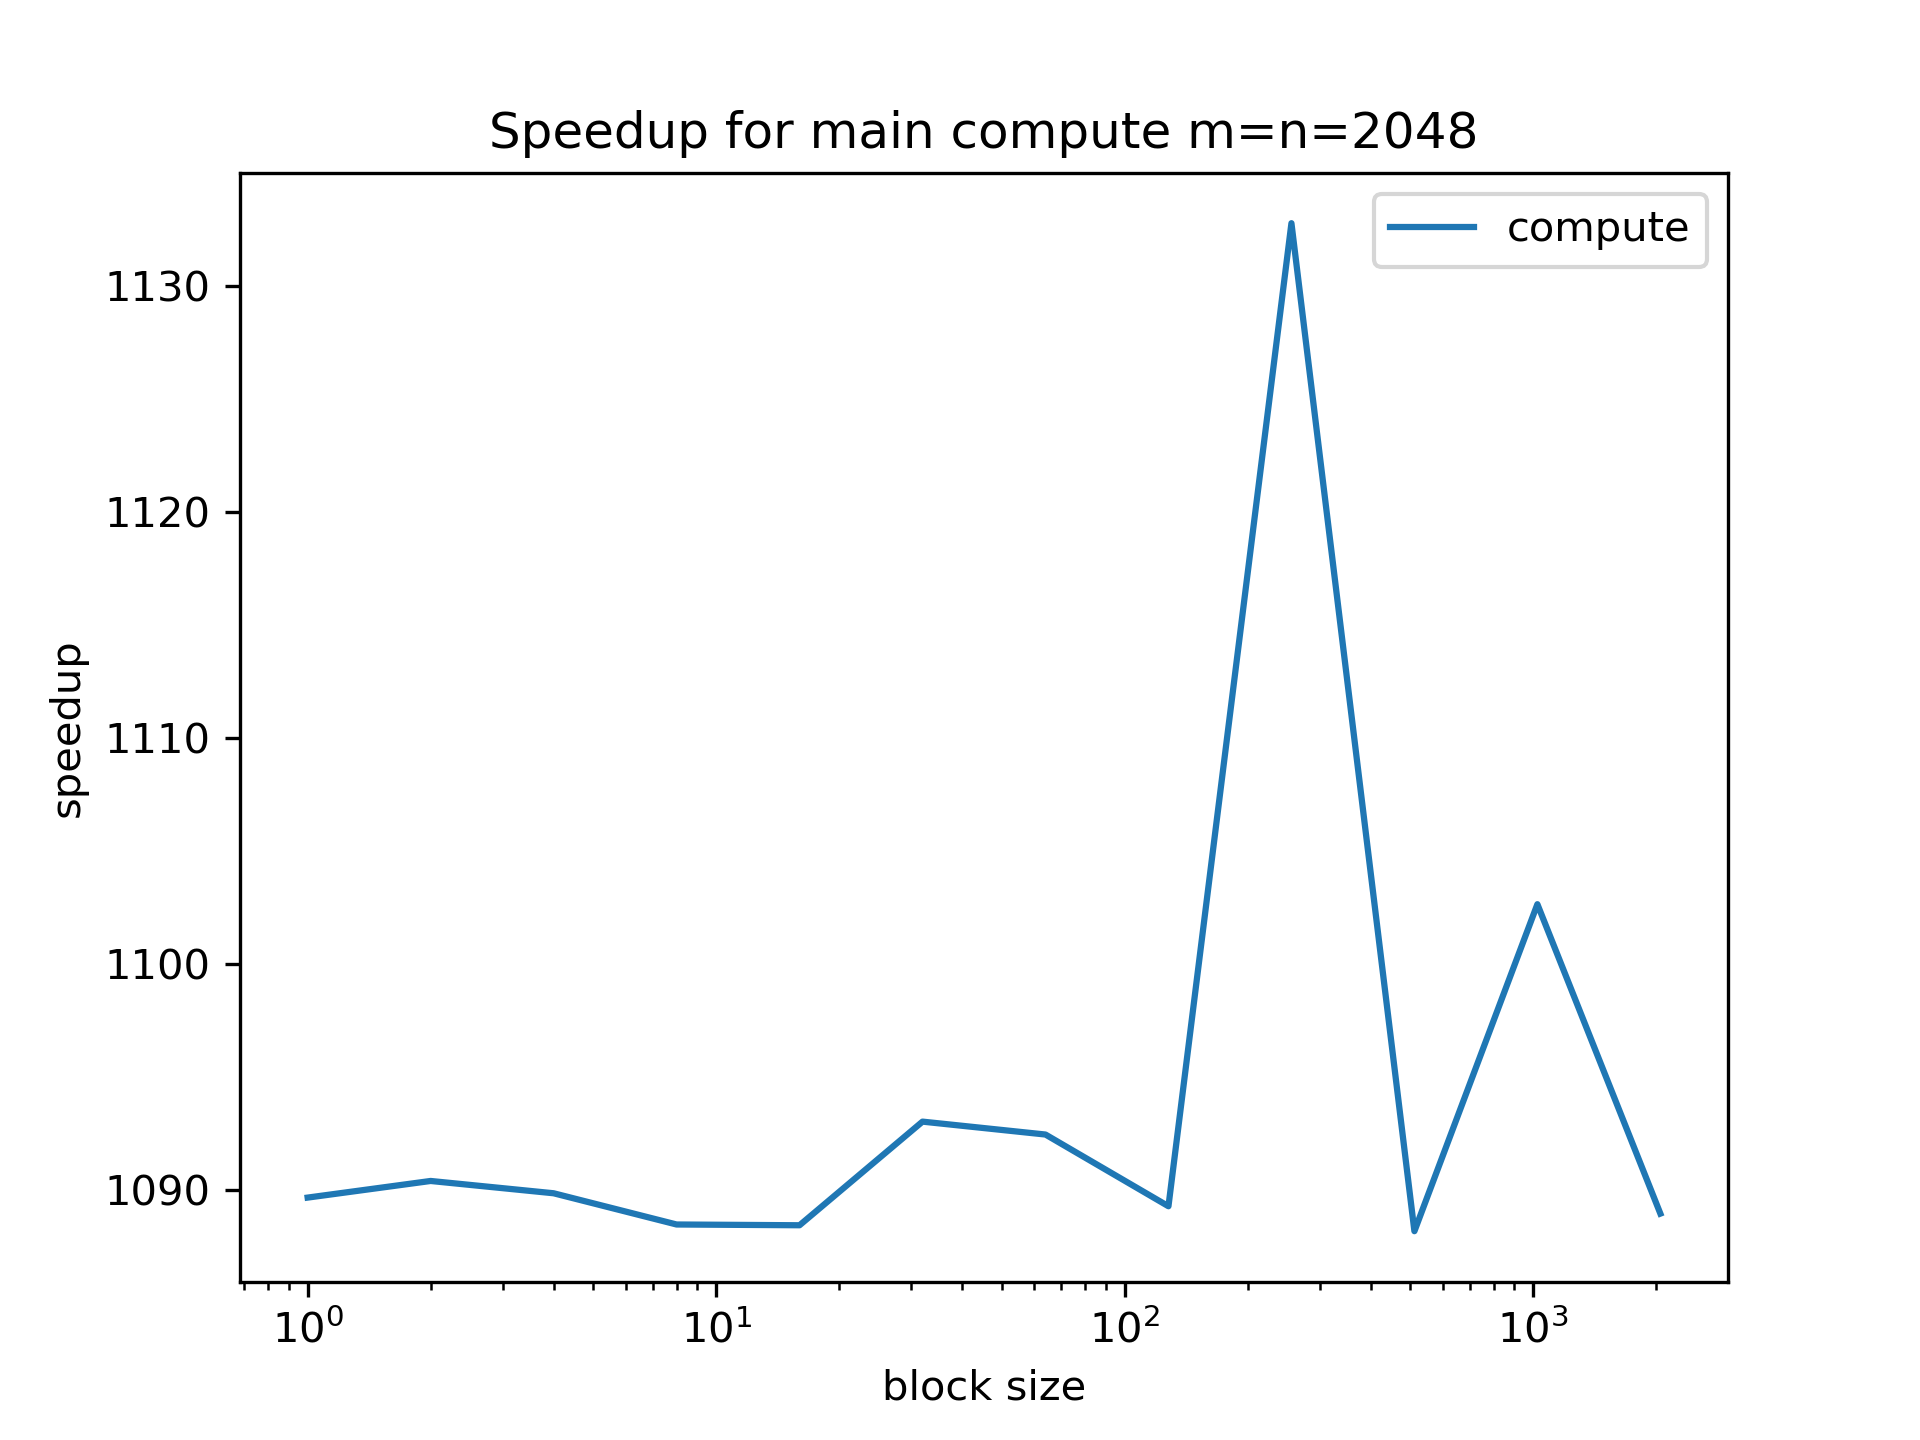
\includegraphics[width=.5\linewidth]{../float/writeup/compute_plot_m2048.png}
		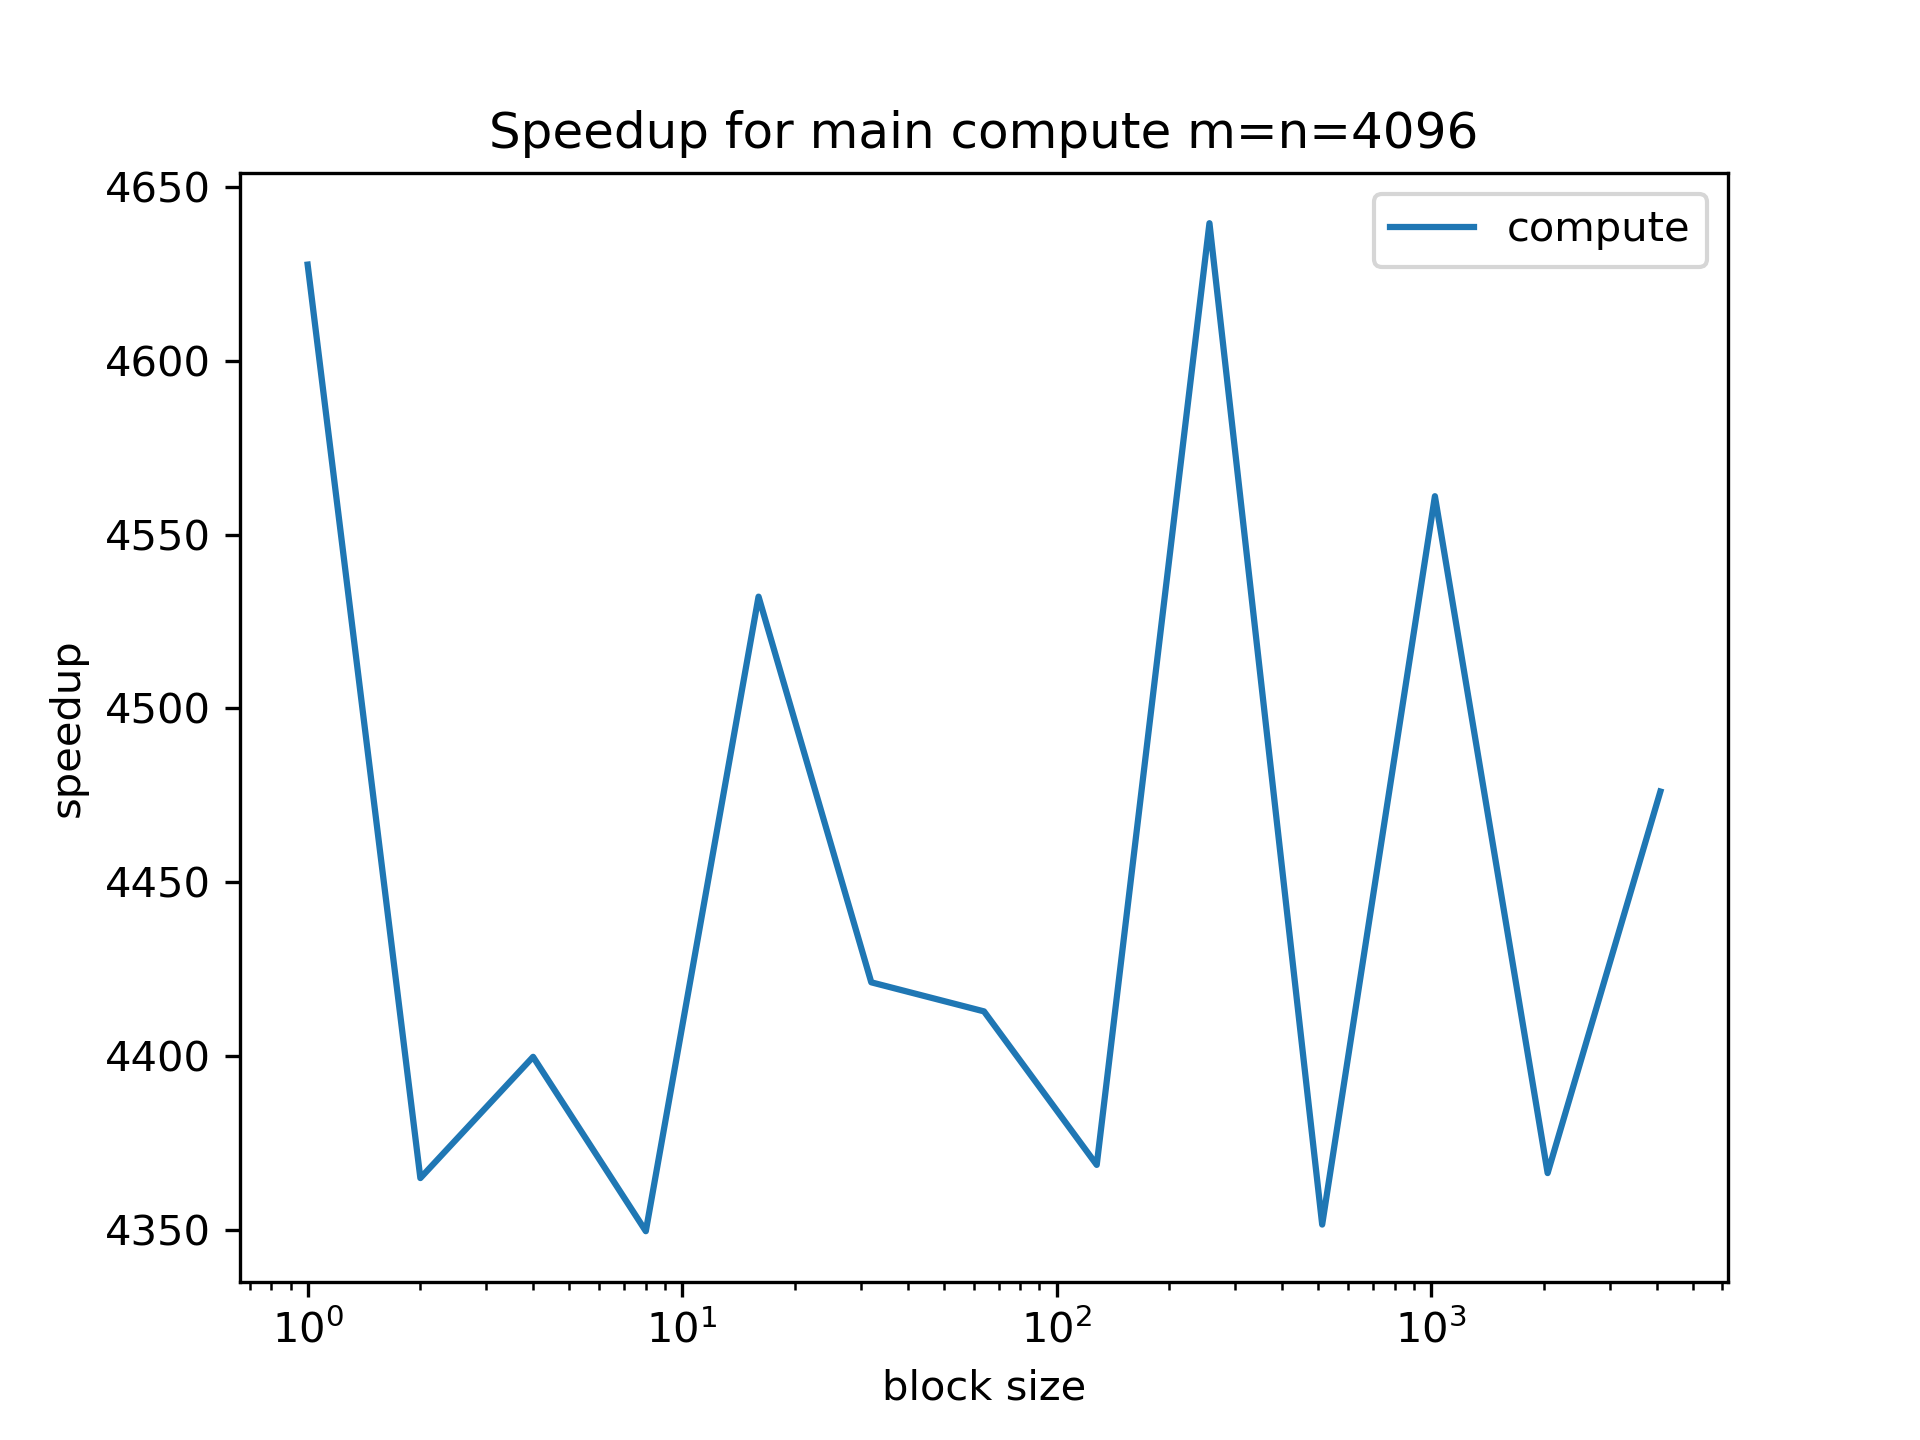
\includegraphics[width=.5\linewidth]{../float/writeup/compute_plot_m4096.png}
		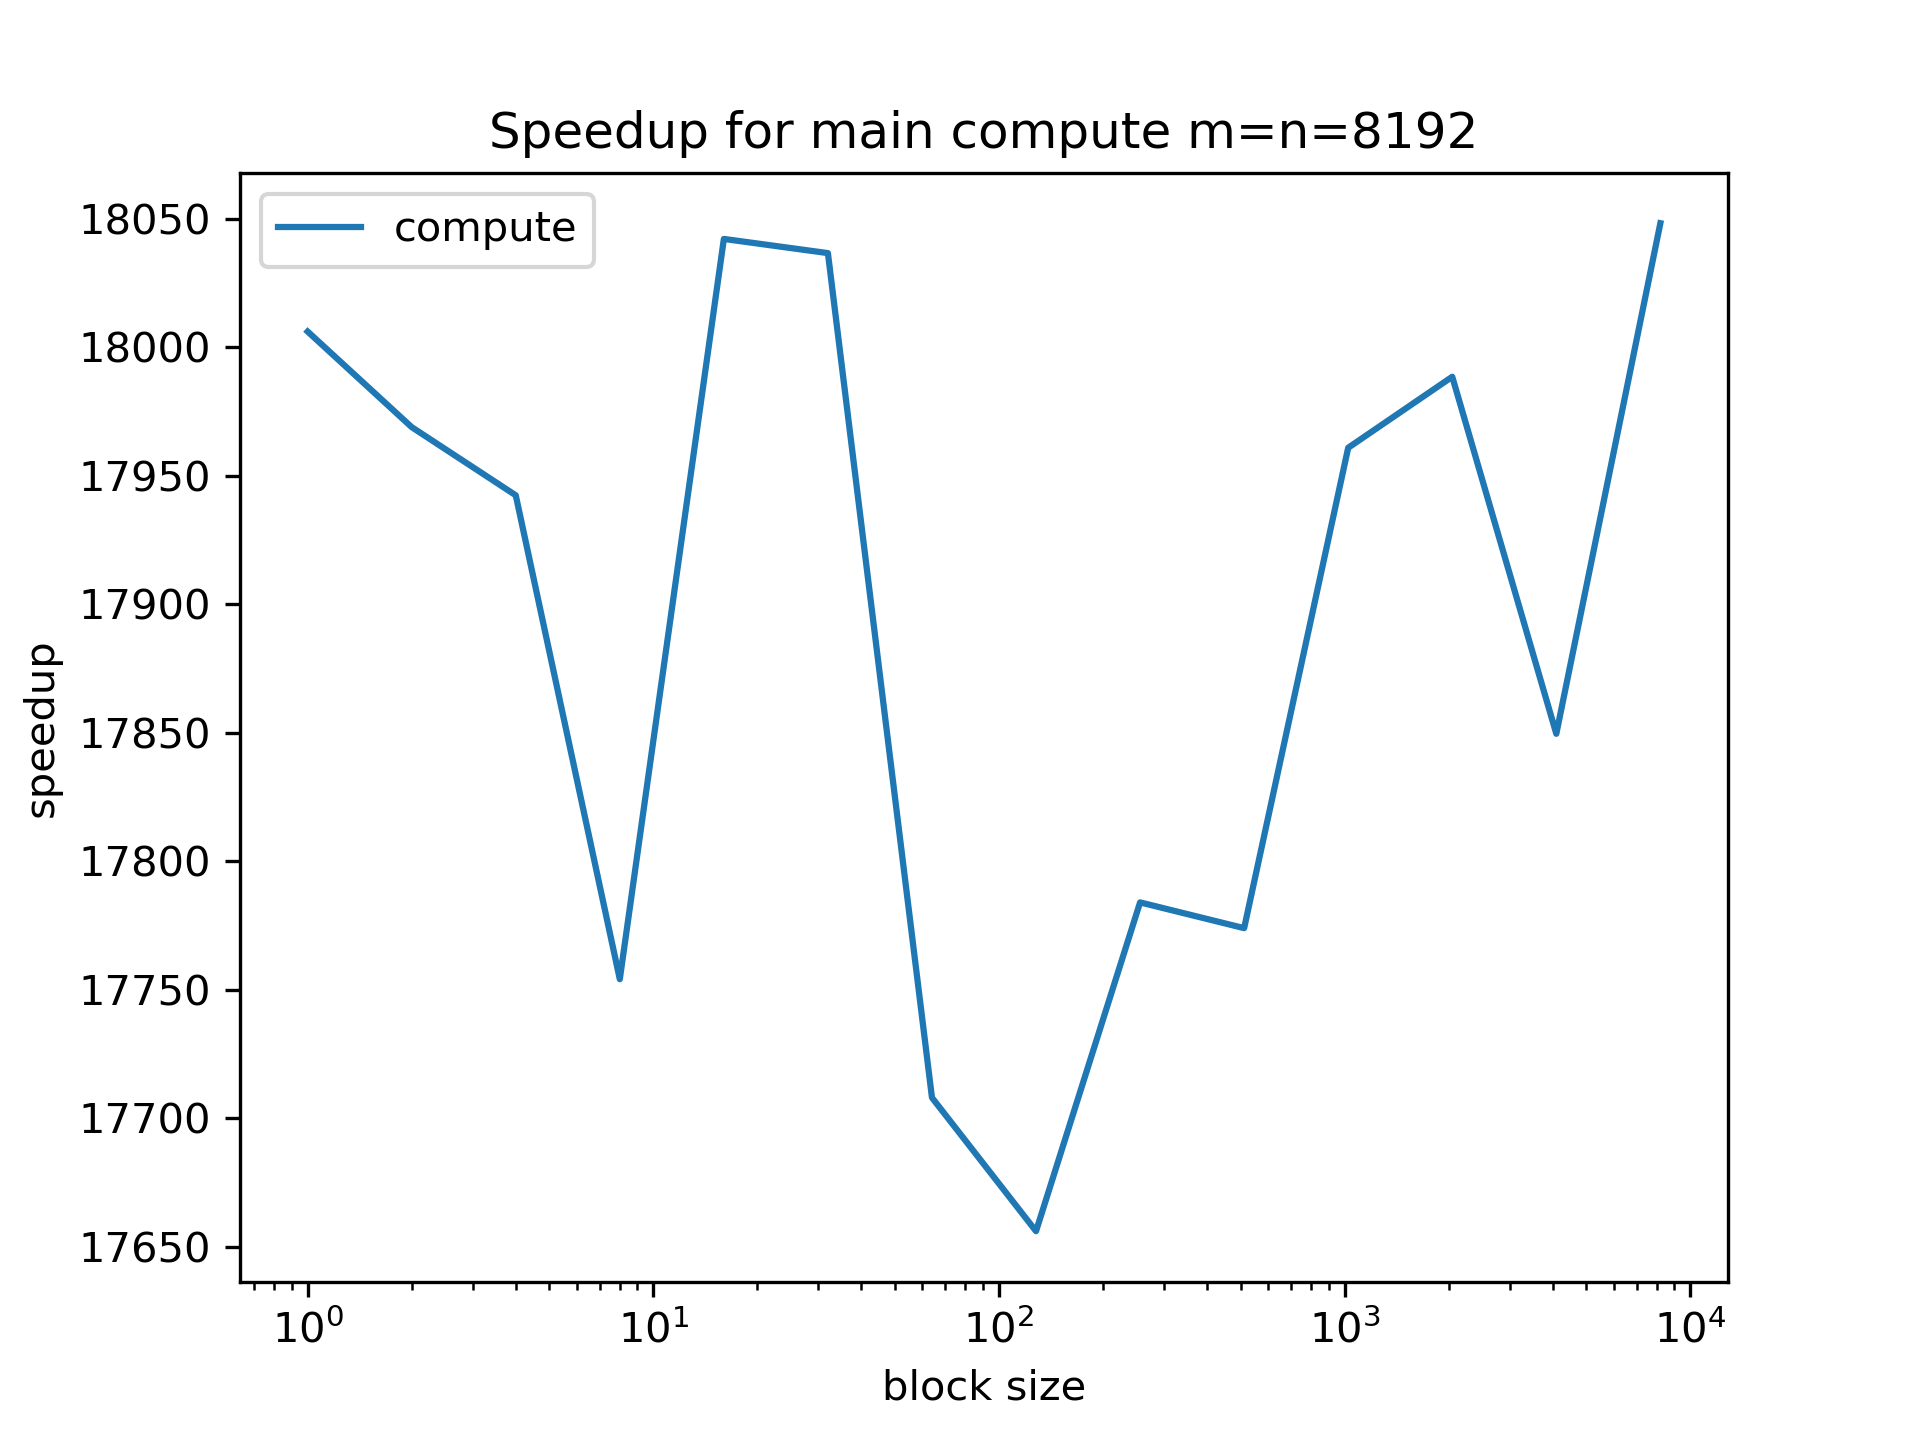
\includegraphics[width=.5\linewidth]{../float/writeup/compute_plot_m8192.png}
		%\label{fig:1}
	\end{figure}


\section{Task3}

	In the figure below I plot the speedup against blocksize for the
	caclulation of the average temperature  compared to using my reduction
	code from homework 1. I

	\begin{figure}[h!]
		\centering
		\includegraphics[width=.5\linewidth]{../float/writeup/reduce_plot_m.1024png}
		\includegraphics[width=.5\linewidth]{../float/writeup/reduce_plot_m.2048png}
		\includegraphics[width=.5\linewidth]{../float/writeup/reduce_plot_m.4096png}
		\includegraphics[width=.5\linewidth]{../float/writeup/reduce_plot_m.8192png}
		%\label{fig:1}
	\end{figure}

\section{Task4}
	
	For this task involving converting the cuda code into double precision I wasnt able
	to completely convert the main iteration loop as surface memory which I was using 
	to store my matrices cant hold double precision numbers easily. Instead I chose to 
	only change the main computation in double precision while storing the results in 
	floating point precision by downcasting the results into floats. Replacing the floats
	with doubles in every other bit of code otherwise worked without much thought.



\bibliographystyle{plain}
\bibliography{refs}

\end{document}

